\documentclass{article}
\usepackage{color}
\usepackage{soul}
\usepackage{multirow}
\usepackage{pgfplots}
\usepackage{ifthen}
\usepackage{tikz}
\usepackage[UTF8]{ctex}
\usepackage[left=2cm,right=2cm,top=2cm,bottom=2cm]{geometry}
\geometry{a4paper}
\usepackage{tikz}
\usetikzlibrary{chains}
\newcommand{\diff}{\mathop{}\!\mathrm{d}}
\usepackage{appendix} 
\usepackage{lipsum}
\usepackage{listings}
\usepackage{diagbox}
\usepackage{pdfpages}
\usepackage{xcolor}
\usepackage{pdflscape}
\usepackage{soul}
\usepackage{booktabs}
\usepackage{longtable}
\usepackage{multirow} 
\usepackage{multicol} 
\usepackage[most]{tcolorbox}
\newtcolorbox{mycolorbox}[1][]{
  sharp corners,
  colback=white, 
  colframe=black, 
  coltext=blue, 
  boxsep=5pt, 
  left=2pt, 
  right=2pt, 
  top=1pt, 
  bottom=1pt,
  breakable,
  #1 
}
\usepackage{subcaption}
\lstset{
    backgroundcolor=\color{gray!20},
    basicstyle=\ttfamily,
    commentstyle=\color{darkgray}\ttfamily,
    stringstyle=\color{red},
    showstringspaces=false,
    numbers=left,
    numberstyle=\tiny\color{gray},
    stepnumber=1,
    numbersep=10pt,
    tabsize=4,
    showspaces=false,
    showtabs=false,
    frame=single,
    captionpos=b,
    breaklines=true,
    breakatwhitespace=false,
    escapeinside={\%*}{*)},
    xleftmargin=\parindent,
    xrightmargin=\parindent,
}
\lstdefinestyle{dockerstyle}{
    language=bash,
    keywordstyle=\color{blue}\bfseries,
    morekeywords={FROM, RUN, CMD, LABEL, EXPOSE, ENV, ADD, COPY, ENTRYPOINT, VOLUME, USER, WORKDIR, ARG, ONBUILD},
}
\lstdefinestyle{pythonstyle}{
    language=Python,
    keywordstyle=\color{blue}\bfseries,
    morekeywords={import, from, as, def, return, class, self, if, elif, else, while, for, try, except, with},
}
\lstdefinestyle{cstyle}{
    language=C,
    keywordstyle=\color{blue}\bfseries,
    morekeywords={size_t, printf},
}
\lstdefinestyle{bashstyle}{
    language=bash,
    keywordstyle=\color{blue}\bfseries,
    morekeywords={if, then, else, fi, for, in, do, done, echo, exit, return, function},
    commentstyle=\color{green}\ttfamily,
}
\usepackage{algorithm}
\usepackage{algpseudocode}
\renewcommand{\algorithmicrequire}{\textbf{Input:}}  
\renewcommand{\algorithmicensure}{\textbf{Output:}}  
\usepackage{amsmath}
\usepackage{amsthm}
\DeclareMathOperator{\sigm}{sigm}
\usepackage{graphicx}
\usepackage{float}
\renewcommand{\vec}[1]{\boldsymbol{#1}}
\usepackage{amssymb}
\usepackage{booktabs} 
\usepackage{hyperref}
\usepackage{titlesec}
\usepackage{caption}
\usepackage{fontspec}
\usepackage{xeCJK}
\setCJKmainfont{SimSun} 
\title{\Huge CUDA\&CUDA和OpenMP混合编程实验报告}
\author{21121178 王士博}
\begin{document}
\maketitle
\section{实验环境}
\textbf{Windows11 Professional 22H2 x64:} \\
\\
\indent \indent \indent \begin{minipage}[H]{0.7\textwidth}
    \begin{itemize}
        \item \textbf{处理器:}Intel(R) Core(TM) i7-11800H CPU @ 4.60GHz 16线程
        \item \textbf{内存:}32.0 GB
        \item \textbf{显卡:}NVIDIA GeForce RTX 3070
        \item \textbf{显卡驱动版本:}11.6
        \item \textbf{编程语言:}C++
        \item \textbf{编译器:}nvcc
        \item \textbf{编程平台:}Visual Studio 2019
    \end{itemize}
\end{minipage}
\section{实验目的}
\begin{enumerate}
    \item 了解CUDA的安装方式和注意问题。通过简洁明了地列出CUDA安装的步骤和关键注意事项,目的在于为CUDA新用户提供一个清晰、易于遵循的安装指南。这不仅帮助用户高效完成CUDA环境的配置,也旨在通过分享实践经验,降低并行编程技术的入门门槛,尤其是对于那些首次尝试在个人计算机上进行CUDA编程的用户。
    \item 使用CUDA或者CUDA和OpenMP混合编程实现矩阵乘法并且根据自己的电脑配置进行优化。现矩阵乘法的CUDA版本以及可能的OpenMP-CUDA混合编程版本,并基于个人机器的具体配置,从多个角度对比其加速比。此实验目的在于探究CUDA和OpenMP-CUDA混合编程技术在执行复杂运算任务时的性能差异,以及评估在不同计算资源配置下的执行效率。通过实验,旨在深入理解GPU并行计算的优势与局限,以及混合编程模式在提升计算性能方面的潜力,同时,通过附上源码,增加实验的可重复性和透明度,为并行计算领域的学习者和研究者提供参考。
\end{enumerate}
\section{实验步骤}
\subsection{CUDA的安装}
\begin{enumerate}
    \item \textbf{下载CUDA Toolkit:}这一步需要区分任务性质,首先确定是进行深度学习还是
    进行CUDA编程,如果只是进行深度学习,那么没没有必要安装完整的CUDA Toolkit,只需使用conda
    在虚拟环境中安装cudatoolkit即可,步骤如(b);如果是进行CUDA编程,那么需要下载完整的CUDA Toolkit如步骤(a)。
    \[
\text{CUDAToolkit} =
\left\{
\begin{array}{ >{\displaystyle}l >{\displaystyle}l }
\text{NVIDIA CUDA Development} & \parbox[t]{5cm}{包含进行CUDA编程所需的库、头文件和编译工具。} \\
\text{NVIDIA CUDA Documentation} & \parbox[t]{5cm}{提供CUDA的官方文档,包括开发者指南、API参考、编程指南等。} \\
\text{NVIDIA CUDA Nsight NVTX} & \parbox[t]{5cm}{性能分析工具,用于标记和组织GPU性能分析的时序事件。} \\
\text{NVIDIA CUDA Runtime} & \parbox[t]{5cm}{包含CUDA运行时库,支持CUDA程序的执行和运行。} \\
\text{NVIDIA CUDA Samples} & \parbox[t]{5cm}{一组演示如何使用CUDA进行编程的示例。} \\
\text{NVIDIA CUDA Visual Studio Integration} & \parbox[t]{5cm}{CUDA与Visual Studio集成的工具和插件。} \\
\text{NVIDIA Nsight Compute} & \parbox[t]{5cm}{用于CUDA应用的性能分析工具,提供深入的硬件级别性能分析。} \\
\text{NVIDIA Nsight Systems} & \parbox[t]{5cm}{系统级性能分析工具,提供全面的系统性能分析,包括CPU和GPU活动。} \\
\end{array}
\right.
\]
\[
\text{Conda cudatoolkit} =
\left\{
\begin{array}{ >{\displaystyle}l >{\displaystyle}l }
\text{NVIDIA CUDA Runtime} & \parbox[t]{5cm}{包含CUDA运行时库,支持CUDA程序的执行和运行。} \\
\text{部分 NVIDIA CUDA Development} & \parbox[t]{5cm}{可能包括一些必要的库和头文件,用于基础的CUDA开发。} \\
\end{array}
\right.
\]
\begin{center}
    \begin{tikzpicture}
        \draw (0,0) ellipse (4cm and 2cm) node[below=1.5cm]{CUDA Toolkit};
        \draw (0,0) ellipse (2.5cm and 1cm) node {cudatoolkit};
        \node at (0, -2.5) {cudatoolkit和CUDA Toolkit包含关系};
    \end{tikzpicture}
\end{center}
    \begin{enumerate}
        \item 访问NVIDIA官网,下载适用于自己操作系统的CUDA Toolkit。下载地址:\url{https://developer.nvidia.com/cuda-toolkit-archive}。
        选择自己的系统相关信息如下图所示:
        \begin{figure}[H]
            \centering
            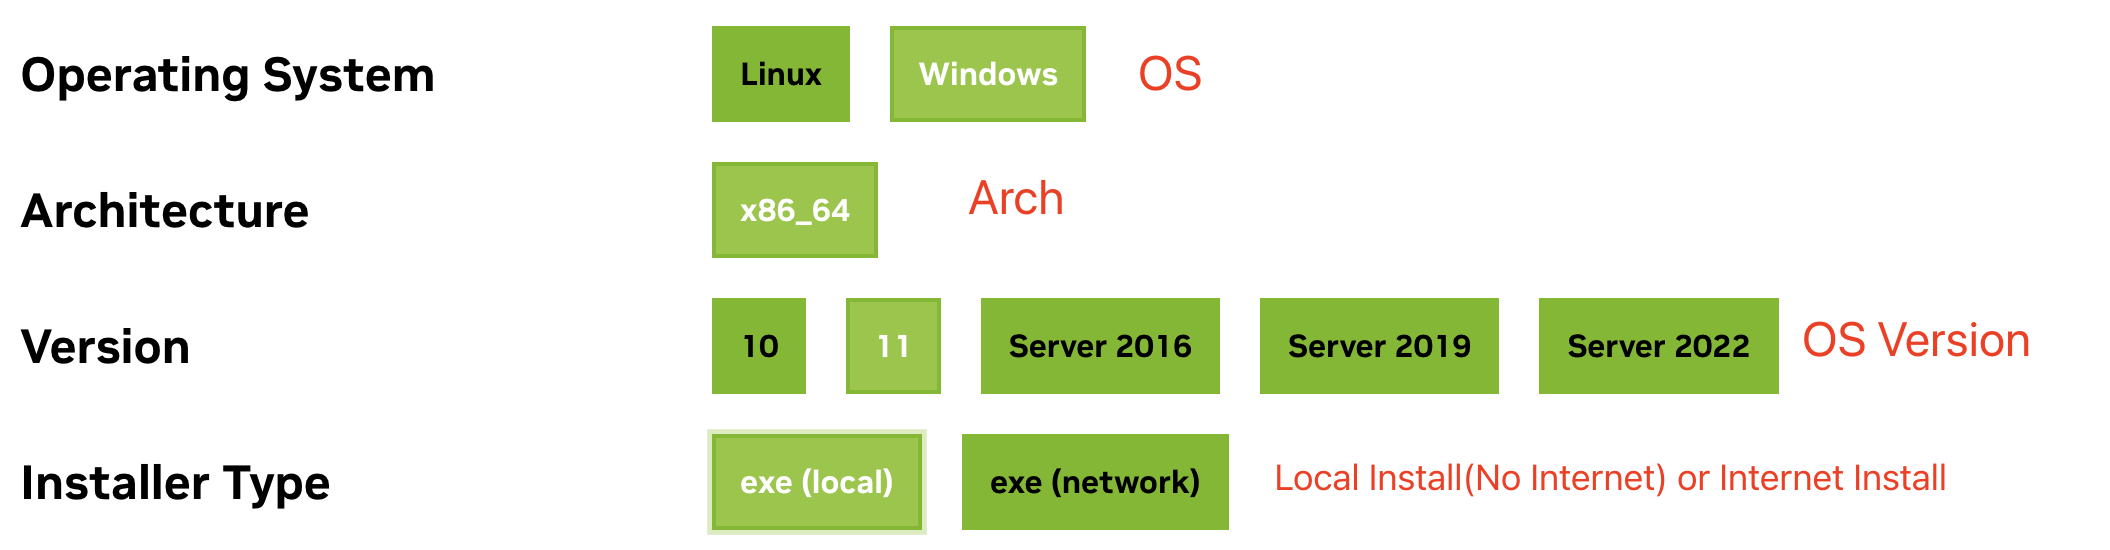
\includegraphics[width=0.8\textwidth]{cudadownload.png}
            \caption{CUDA Toolkit下载}
        \end{figure}
        \item 打开\url{https://anaconda.org/},搜索cudatoolkit,找到Pytorch/Tensorflow需要的
        cudatoolkit版本,然后进复制下载命令进行下载比如下面下载11.6版本的cudatoolkit。
        \begin{lstlisting}[style=bashstyle]
conda install deepmodeling::cudatoolkit
        \end{lstlisting}
    \end{enumerate}
    \item 运行刚刚下载可执行文件,全部默认安装即可,如果不在C盘安装会出现一些问题,有的程序会默认
    去C盘找CUDA的驱动文件导致无法运行。Linux不分盘所以无所谓。
    \item 安装完成后,需要配置环境变量,需要配置如下有名称的环境变量:
    \begin{lstlisting}[style=bashstyle]
CUDA_PATH = C:\Program Files\NVIDIA GPU Computing Toolkit\CUDA\v11.6
CUDA_PATH_V11_6 = C:\Program Files\NVIDIA GPU Computing Toolkit\CUDA\v11.6
    \end{lstlisting}
    和下面Path变量中的条目:
    \begin{lstlisting}[style=bashstyle]
C:\Program Files\NVIDIA GPU Computing Toolkit\CUDA\v11.6\bin
C:\Program Files\NVIDIA GPU Computing Toolkit\CUDA\v11.6\libnvvp
    \end{lstlisting}
    其中一个系统中可以有多个驱动版本,如果你想要使用什么版本,可以修改\texttt{CUDA\_PATH}
    以及将Path中的相应版本的路径上移到所有版本的路径之上即可实现快速的CUDA版本切换。
    \item 这时已经基本配置完成,\texttt{win+R}输入\texttt{powershell}打开powershell,
    输入下面的指令和看到下面输出的结果之后,说明CUDA已经安装成功。
    \begin{lstlisting}[style=bashstyle]
(base) PS C:\Users\24692> nvcc -V
nvcc: NVIDIA (R) Cuda compiler driver
Copyright (c) 2005-2021 NVIDIA Corporation
Built on Fri_Dec_17_18:28:54_Pacific_Standard_Time_2021
Cuda compilation tools, release 11.6, V11.6.55
Build cuda_11.6.r11.6/compiler.30794723_0
(base) PS C:\Users\24692> nvidia-smi
Mon Apr  8 09:38:47 2024
NVIDIA-SMI 551.86   Driver Version: 551.86    CUDA Version: 12.4   
    \end{lstlisting}
    这里的CUDA Version和CUDA Toolkit的版本不一样是因为这里的CUDA Version是显卡支持的
    最高CUDA版本,而CUDA Toolkit是你安装的CUDA版本。
    \item 按需安装cuDNN,cuDNN是深度学习底层的算子库,为一些深度学习中的基本运算提供加速。
\end{enumerate}
\subsection{Ablation Study}
本实验将这里的矩阵乘法任务分为下面两个子任务:
\begin{itemize}
    \item \textbf{数据的初始化:}相乘的两个矩阵的随机数初始化的阶段。
    \item \textbf{矩阵乘法:}两个矩阵相乘的阶段(CUDA编程还包括将数据复制回主存的时间)。
\end{itemize}
然后本实验针对上面这两个阶段进行编程的设计。其中数据的初始化需要两层循环进行初始化,但是
可以预见到,这里的两层循环的任务是可以并行的,因为每个矩阵元素的初始化操作都是独立的。
所以这里可以使用\texttt{\#pragma omp parallel for collapse}进行并行化。而矩阵
乘法的阶段的最后结果的每一个元素的计算都是相互独立的,所以可以并行计算,这里可以使用OpenMP
和CUDA进行并行化计算。实验的源代码可以见附录。

\begin{table}[H]
    \centering
    \begin{tabular}{|c|c|c|c|c|c|c|}
        \hline
        Config & 1 & 2 & 3 & 4 & 5 & 6 \\
        \hline
        init omp & - & True & - & - & True & True\\
        \hline
        cal omp & - & - & True & - & True & - \\
        \hline
        cal gpu & - & - & - & True & - & True \\
        \hline
        1 & 2.67 & 2.75 & 0.46 & 0.0816 & 0.48 & 0.1912 \\
        2 & 2.66 & 2.77 & 0.47 & 0.0812 & 0.47 & 0.1855 \\
        3 & 2.70 & 2.76 & 0.45 & 0.0742 & 0.49 & 0.1852 \\
        4 & 2.67 & 2.73 & 0.47 & 0.0788 & 0.47 & 0.1901 \\
        5 & 2.66 & 2.77 & 0.46 & 0.0796 & 0.47 & 0.1935 \\
        \hline
        ave & 2.67200 & 2.75600 & 0.46200 & 0.07908 & 0.47600 & 0.18910\\
        \hline
        SpeedUp & - & 0.969521 & 5.783550 & 33.788569 & 5.613445 & 14.130090 \\
        \hline
    \end{tabular}
    \caption{Ablation Of Matrix Sized 1000(s)}
    \label{tab:1}
\end{table}
\begin{table}[H]
    \centering
    \begin{tabular}{|c|c|c|c|c|c|c|}
        \hline
        Config & 1 & 2 & 3 & 4 & 5 & 6 \\
        \hline
        init omp & - & True & - & - & True & True\\
        \hline
        cal omp & - & - & True & - & True & - \\
        \hline
        cal gpu & - & - & - & True & - & True \\
        \hline
        1 & 32.65 & 34.13 & 5.67 & 0.3685 & 5.78 & 0.1695\\
        2 & 31.95 & 32.15 & 5.62 & 0.3670 & 5.69 & 0.1718\\
        3 & 32.01 & 32.70 & 5.70 & 0.3702 & 5.67 & 0.1909 \\
        4 & 32.20 & 32.22 & 5.64 & 0.3764 & 5.79 & 0.2055 \\
        5 & 31.97 & 33.20 & 5.66 & 0.3718 & 5.90 & 0.1749 \\
        \hline
        ave & 32.15600 & 32.88000 & 5.65800 & 0.37078 & 5.76600 & 0.18252\\
        \hline
        SpeedUp & - & 0.977981 & 5.683280 & 86.725282 & 5.576830 & 176.177953\\
        \hline
    \end{tabular}
    \caption{Ablation Of Matrix Sized 2000(s)}
    \label{tab:2}
\end{table}
\begin{table}[H]
    \centering
    \begin{tabular}{|c|c|c|c|c|c|c|}
        \hline
        Config & 1 & 2 & 3 & 4 & 5 & 6 \\
        \hline
        init omp & - & True & - & - & True & True\\
        \hline
        cal omp & - & - & True & - & True & - \\
        \hline
        cal gpu & - & - & - & True & - & True \\
        \hline
        1 & 146.68 & 158.80 & 21.79 & 0.9331 & 22.01 & 0.5067\\
        2 & 143.14 & 144.90 & 21.66 & 0.9471 & 21.90 & 0.5045\\
        3 & 144.12 & 144.10 & 21.63 & 0.9199 & 21.80 & 0.4886\\
        4 & 143.30 & 146.13 & 21.88 & 0.9233 & 21.89 & 0.5018\\
        5 & 144.22 & 145.32 & 21.70 & 0.9545 & 22.02 & 0.4909\\
        \hline
        ave & 144.292 & 147.85 & 21.732 & 0.93558 & 21.924 & 0.4985 \\
        \hline
        SpeedUp & - & 0.976 & 6.64 & 154.23 & 6.58 & 289.45\\
        \hline
    \end{tabular}
    \caption{Ablation Of Matrix Sized 3000(s)}
    \label{tab:3}
\end{table}
通过上面的消融实验的数据,可以得到下面的结果:
\begin{enumerate}
    \item GPU的有效加速:使用GPU对矩阵乘法这种高密度高并行高独立性的计算的提升是巨大的,可以从表\ref{tab:1}表\ref{tab:2}
    表\ref{tab:3}中看出,从一开始的1000大小矩阵的加速比33.79到最后的3000大小矩阵的加速比289.45(相比
    于基线数据),其中相比于其他的并行化操作,比如只使用OpenMP优化乘法,同时使用OpenMP优化初始化和乘法也有着
    较为明显的加速。
    可以看出越大规模的矩阵运算,GPU的加速效果越高,具体的原因分析有下:
    \begin{enumerate}
        \item \textbf{并行计算能力}
        \begin{itemize}
          \item 硬件架构优势:CUDA基于NVIDIA的GPU(图形处理单元)设计,而GPU含有成百上千个核心,能够同时执行成千上万的线程。这种大规模并行处理能力使得GPU非常适合执行数据并行任务,如矩阵乘法。
          \item 数据并行:在矩阵乘法中,计算每个输出元素的操作是独立的。CUDA能够将这些操作分布到多个线程中并行执行,显著减少总的计算时间。
        \end{itemize}
      
        \item \textbf{内存带宽}
        \begin{itemize}
          \item 高内存带宽:GPU具有非常高的内存带宽,能够更快地读写数据,这对于数据密集型的计算任务(如矩阵乘法)尤其重要,因为矩阵乘法需要频繁地访问内存中的数据。
        \end{itemize}
      
        \item \textbf{优化的内存访问}
        \begin{itemize}
          \item 共享内存和缓存:CUDA允许开发者使用GPU上的共享内存,这是一种低延迟、高带宽的内存。合理利用共享内存可以减少对全局内存的访问次数,提高数据访问效率。此外,通过优化内存访问模式(如合并内存访问和避免内存冲突),可以进一步提高性能。
        \end{itemize}
      
        \item \textbf{加速比和并行计算效率}
        \begin{itemize}
          \item 并行加速比通常用来衡量并行程序相比于串行版本的性能提升,定义为:
          $ 加速比 = \frac{串行执行时间}{并行执行时间} $
          \item 对于矩阵乘法,随着矩阵大小的增加,串行执行时间增长的速度远快于并行执行时间的增长。这是因为,并行计算的开销(如线程创建和管理、数据传输等)相对于整体计算量来说,随着问题规模的扩大变得不那么重要。
          \item Amdahl定律:它描述了系统中固定部分对加速比的限制。在完全并行化的矩阵乘法中,理论上这部分很小,但实际上随着矩阵大小的增加,可并行化的部分占比增加,从而实现更高的加速比。
          \item Gustafson定律:它强调了随着数据规模的增加,绝对加速比可以提高。对于大规模矩阵乘法,这意味着并行计算可以利用更多的硬件资源,实现更高的性能提升。
        \end{itemize}
      \end{enumerate}
      \item 使用OpenMP不一定会产生加速:从上面可以看出使用OpenMP并行优化数据的初始化并不一定能
      带来很明显的加速效果。其中只使用OpenMP并行优化数据初始化操作对比普通的串行程序来看加速比并不高,甚至还
      低于1,这是因为OpenMP的并行化操作也会带来一些额外的时间开销,这些时间开销可能会抵消掉OpenMP并行化
      优化的时间。在只使用OpenMP优化乘法操作以及同时使用OpenMP优化初始化和乘法操作的对比中,也不是很明显
      。更加明显的是只有GPU加速乘法以及OpenMP加速初始化和GPU优化乘法,这两组对比中可以看出,在1000大小的
      矩阵上OpenMP居然出现了负优化的现象,但是在后续的2000大小和3000大小矩阵中却有着明显的加速效果,
      可以总结为以下几点:
      \begin{enumerate}
        \item \textbf{OpenMP并行化开销:}可以看出,如果本身的操作速度已经很快,那么没有必要
        一定要生搬硬套OpenMP,OpenMP启动并行化会有额外的开销,如果这种开销大于并行化所带来的加速
        效果,那么使用OpenMP只能是得不偿失,会对程序产生负优化,很好的例子就是1000大小矩阵
        表\ref{tab:1}中单独GPU加速乘法以及使用OpenMP优化初始化和GPU加速乘法的负优化的例子。
        从这里也可以总结出OpenMP应该使用的场景。如果一个场景有很多的串行算法模块,$O(1),O(n)
        ,O(n^2),o(n^3) \dots O(n^x)$,那么就需要使用OpenMP并行化处理高复杂度的算法模块
        (如果可以的话,要求算法模块内部有一定的无关性),并且前提是$T_{parallel cost}>T(algorithm_{O(n^x)})$
        ,如果OpenMP的并行化开销大于任何一个模块的优化的时间,那么所有的优化都是没有意义的,
        并且使用OpenMP优化复杂度高的算法,降低复杂度,这样使得总体的复杂度降低,以此来进行加速。
        \item \textbf{普通的程序的瓶颈不仅在CPU而且在访存:}为什么串行程序和OpenMP优化矩阵
        乘法加上OpenMP优化初始化的加速比都没有显著的提升,并且GPU在加上了初始化的OpenMP优化
        会产生越来越大的初始化操作,一方面的原因是因为GPU的并行化远高于GPU,另一点是普通的
        程序在使用大量的时间在访存上。访存时间成为了程序的瓶颈,再怎么使用OpenMP开多线程也没有什么作用
        都要停止等待内存数据搬运到GPU。并且GPU加上OpenMP优化初始化的加速比随着矩阵大小越来越大,
        这说明,GPU没有访存的高额开销,瓶颈就是在初始化的优化程度上。
      \end{enumerate}
\end{enumerate}

\section{实验感想}
通过这次实验,我对GPU计算的潜力和并行计算的效率有了更深刻的认识。通过做实验记录数据,我了解了GPU在处理矩
阵乘法这类高度并行化的任务上,相较于传统CPU具有显著的加速优势。通过了消融实验,我被GPU架
构带来的硬件优势和内存带宽的高效利用所震撼。CUDA技术真正实现了通过并行处理大幅度减少计算时间的可
能性,而这一点在规模更大的矩阵乘法中表现得尤为明显。

在进行OpenMP并行化时,实验教会了我并行化是一把双刃剑。OpenMP的引入并不总是能带来性能上的提升,有时
它的并行化开销甚至可能导致性能的下降。尤其在处理较小规模的数据时,OpenMP的加速效果并不明显,这提
示我们在决定使用并行计算时,必须考虑到算法的复杂性和计算负担。

此外,我也意识到,普通程序的访存操作在串行计算中占据了大量的时间,成为性能提升的瓶颈。而GPU的高效计算
能力和内存操作显然突破了这一限制,尤其是在矩阵规模增大时,GPU计算的优势更加凸显。我认为,理解和合
理利用硬件特性对于优化程序性能至关重要。

总之,这次实验不仅加深了我对并行计算技术的理解,而且也让我更加清晰地认识到了在实际应用中如何根据计
算任务的特点和规模来选择合适的优化策略。这将对我未来在计算机科学和深度学习领域的学习和研究提供极大的帮助。
\newpage
\appendix
\section{源代码}
\begin{lstlisting}[style=cstyle,caption={OpenMP和CUDA混合编程}]
#include <iostream>
#include <cstdlib>
#include <cuda_runtime.h>
#include <omp.h>

#define TILE_SIZE 16
#define BLOCK_SIZE 16

__global__ void MatrixMulCUDA(int* A, int* B, int* C, int N) {
    int ROW = blockIdx.y * blockDim.y + threadIdx.y;
    int COL = blockIdx.x * blockDim.x + threadIdx.x;
    int tmpSum = 0;

    if (ROW < N && COL < N) {
        for (int i = 0; i < N; i++) {
            tmpSum += A[ROW * N + i] * B[i * N + COL];
        }
    }
    C[ROW * N + COL] = tmpSum;
}

int main() {
    int sizes[] = { 1000, 2000, 3000 };
    int numSizes = sizeof(sizes) / sizeof(sizes[0]);

    for (int n = 0; n < numSizes; n++) {
        int N = sizes[n];
        size_t bytes = N * N * sizeof(int);

        int* A, * B, * C;
        int* d_A, * d_B, * d_C;

        // 记录开始时间
        double start = omp_get_wtime();

        A = (int*)malloc(bytes);
        B = (int*)malloc(bytes);
        C = (int*)malloc(bytes);

#pragma omp parallel for collapse(2)
        for (int i = 0; i < N; i++) {
            for (int j = 0; j < N; j++) {
                A[i * N + j] = rand() % 10;
                B[i * N + j] = rand() % 10;
            }
        }

        cudaMalloc(&d_A, bytes);
        cudaMalloc(&d_B, bytes);
        cudaMalloc(&d_C, bytes);
        cudaMemcpy(d_A, A, bytes, cudaMemcpyHostToDevice);
        cudaMemcpy(d_B, B, bytes, cudaMemcpyHostToDevice);
        dim3 threadsPerBlock(BLOCK_SIZE, BLOCK_SIZE);
        dim3 blocksPerGrid((N + BLOCK_SIZE - 1) / BLOCK_SIZE, (N + BLOCK_SIZE - 1) / BLOCK_SIZE);
        MatrixMulCUDA << <blocksPerGrid, threadsPerBlock >> > (d_A, d_B, d_C, N);
        cudaDeviceSynchronize();
        cudaMemcpy(C, d_C, bytes, cudaMemcpyDeviceToHost);
        double end = omp_get_wtime();
        std::cout << "Total execution time for " << N << "x" << N << " matrix: " << (end - start) * 1000 << " milliseconds" << std::endl;
        cudaFree(d_A);
        cudaFree(d_B);
        cudaFree(d_C);
        free(A);
        free(B);
        free(C);
    }
    return 0;
}    
\end{lstlisting}
\end{document}